
\documentclass[tikz, border=10mm]{standalone}
\usepackage{xcolor}
\usepackage{tikz}
\usetikzlibrary{positioning, calc, backgrounds, quotes, arrows.meta}

% Color Definitions (Comprehensive List from nn_blocks.tex & pnn_header.tex.j2)
\definecolor{ConvColor}{rgb}{0.98,0.81,0.69} % Apricot
\definecolor{PoolColor}{rgb}{0.8,0.33,0.33}  % Pink/Red
\definecolor{UnpoolColor}{rgb}{0.6,0.7,0.9}  % Blue/Purple
\definecolor{ResBlockColor}{rgb}{0.85,0.92,1.0} % Light Blue
\definecolor{OpColor}{rgb}{0.5,1.0,0.5}      % Green
\definecolor{FcColor}{rgb}{0.6,0.2,0.8}      % Purple
\definecolor{SoftmaxColor}{rgb}{0.9,0.9,0.6} % Yellowish
\definecolor{SumColor}{rgb}{0.9,0.9,0.9}     % Gray
\definecolor{EmbedColor}{rgb}{0.95,0.95,0.8} % Light Yellow
\definecolor{TransColor}{rgb}{0.8,0.9,0.8}   % Light Green

% 3D Style Approximation
\tikzset{
    box3d/.style={
        shape=rectangle,
        draw=black!50,
        fill=#1,
        minimum width=1cm,
        minimum height=1.5cm,
        append after command={
            \pgfextra{
                \draw[fill=#1!80!black, draw=black!50] (\tikzlastnode.north east) -- ++(0.3,0.3) -- ++(-1,0) -- (\tikzlastnode.north west) -- cycle;
                \draw[fill=#1!60!black, draw=black!50] (\tikzlastnode.north east) -- ++(0.3,0.3) -- ++(0,-1.5) -- (\tikzlastnode.south east) -- cycle;
            }
        }
    }
}

\begin{document}
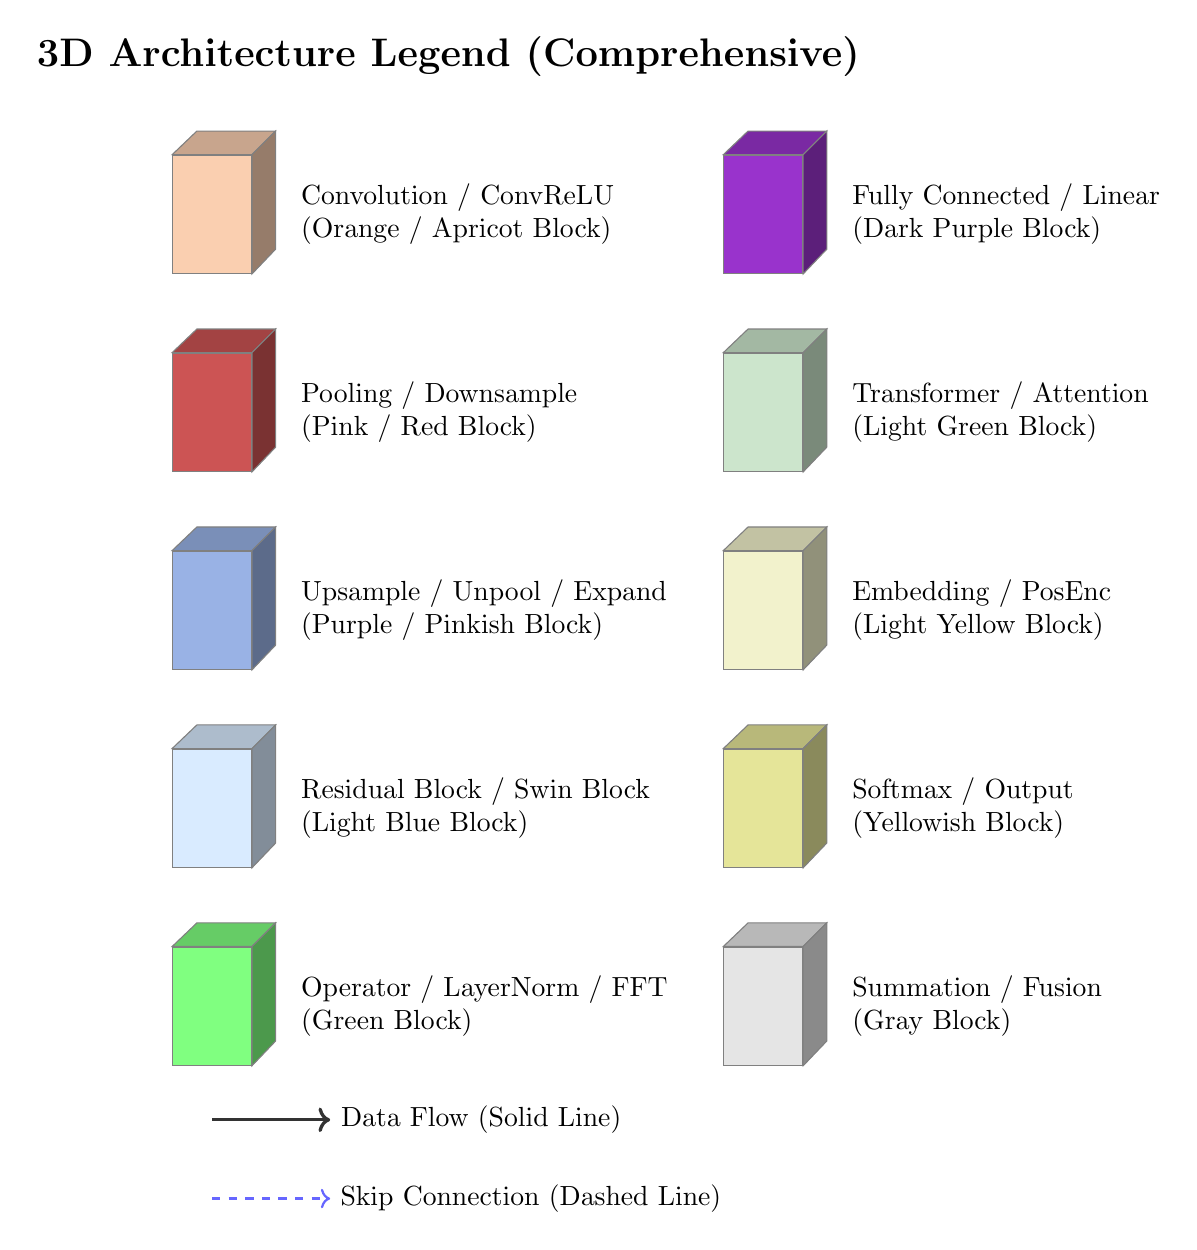
\begin{tikzpicture}[node distance=0.8cm, every node/.style={transform shape}]

% Title
\node[font=\Large\bfseries] at (3, 9) {3D Architecture Legend (Comprehensive)};

% Column 1
\coordinate (col1) at (0, 7);

\node[box3d=ConvColor] (l_conv) at (col1) {};
\node[right=0.5cm of l_conv, align=left] {Convolution / ConvReLU\\(Orange / Apricot Block)};

\node[box3d=PoolColor, below=1.0cm of l_conv] (l_pool) {};
\node[right=0.5cm of l_pool, align=left] {Pooling / Downsample\\(Pink / Red Block)};

\node[box3d=UnpoolColor, below=1.0cm of l_pool] (l_up) {};
\node[right=0.5cm of l_up, align=left] {Upsample / Unpool / Expand\\(Purple / Pinkish Block)};

\node[box3d=ResBlockColor, below=1.0cm of l_up] (l_res) {};
\node[right=0.5cm of l_res, align=left] {Residual Block / Swin Block\\(Light Blue Block)};

\node[box3d=OpColor, below=1.0cm of l_res] (l_op) {};
\node[right=0.5cm of l_op, align=left] {Operator / LayerNorm / FFT\\(Green Block)};

% Column 2
\coordinate (col2) at (7, 7);

\node[box3d=FcColor] (l_fc) at (col2) {};
\node[right=0.5cm of l_fc, align=left] {Fully Connected / Linear\\(Dark Purple Block)};

\node[box3d=TransColor, below=1.0cm of l_fc] (l_trans) {};
\node[right=0.5cm of l_trans, align=left] {Transformer / Attention\\(Light Green Block)};

\node[box3d=EmbedColor, below=1.0cm of l_trans] (l_embed) {};
\node[right=0.5cm of l_embed, align=left] {Embedding / PosEnc\\(Light Yellow Block)};

\node[box3d=SoftmaxColor, below=1.0cm of l_embed] (l_soft) {};
\node[right=0.5cm of l_soft, align=left] {Softmax / Output\\(Yellowish Block)};

\node[box3d=SumColor, below=1.0cm of l_soft] (l_sum) {};
\node[right=0.5cm of l_sum, align=left] {Summation / Fusion\\(Gray Block)};

% Arrows (Bottom)
\coordinate (l_arrow) at (0, -4.5);
\draw[->, very thick, draw=black!80, rounded corners=0.2cm] (l_arrow) -- ++(1.5, 0) node[right, align=left] {Data Flow (Solid Line)};

\coordinate (l_skip) at ($(l_arrow) + (0, -1)$);
\draw[->, dashed, draw=blue!60, thick] (l_skip) -- ++(1.5, 0) node[right, align=left] {Skip Connection (Dashed Line)};

\end{tikzpicture}
\end{document}
